\documentclass{report}
\usepackage[utf8]{inputenc}
\usepackage[T1]{fontenc}
\usepackage[french]{babel}
\usepackage{geometry}
\usepackage{fancyhdr}
\setlength{\headheight}{13pt}
\usepackage{lastpage}
\usepackage{titlesec}
\usepackage{listings}
\usepackage{enumitem}
\usepackage{color}
\usepackage[table]{xcolor}
\usepackage{soul}
\usepackage{graphicx}
\usepackage{amsmath}
\usepackage{amssymb}
\usepackage{hyperref}
\hypersetup{hidelinks}
\usepackage{tikz}
\usetikzlibrary{positioning, shapes.geometric, arrows.meta, calc, fit, backgrounds, shadows}
\usepackage{rotating}
\usepackage{longtable}
\usepackage{array}
\usepackage{float}

\newcommand{\DocName}{OPTIMISATION DE MODELES NEURONAUX A OSCILLATEURS COUPLÉS - RAPPORT FINAL}
\newcommand{\DocAuthors}{\bsc{Da Silva} Tristan - \bsc{Battaglia} Charles-Antoine \\ \bsc{Botté-Magalhaes} Jules - \bsc{Gauthier} Keanu - \bsc{Fraysse} Ianis}

% ===== Couleurs communes =====
\definecolor{dkgreen}{rgb}{0,0.6,0}
\definecolor{gray}{rgb}{0.5,0.5,0.5}
\definecolor{mauve}{rgb}{0.58,0,0.82}
\definecolor{addrred}{rgb}{0.93,0.43,0.43}
\definecolor{commentgray}{rgb}{0.45,0.45,0.45}

% Palette du schéma conceptuel (L1)
\definecolor{hubbg}{RGB}{23,48,77}
\definecolor{hubborder}{RGB}{23,48,77}
\definecolor{hubrule}{RGB}{150,178,206}
\definecolor{cardink}{RGB}{33,41,54}
\definecolor{cardline}{RGB}{160,172,186}
\definecolor{whyborder}{RGB}{31,92,139}
\definecolor{whybg}{RGB}{243,248,252}
\definecolor{whatborder}{RGB}{34,116,80}
\definecolor{whatbg}{RGB}{243,250,246}
\definecolor{howborder}{RGB}{181,84,39}
\definecolor{howbg}{RGB}{253,247,243}
\definecolor{outborder}{RGB}{104,72,140}
\definecolor{outbg}{RGB}{249,246,253}
\definecolor{defiborder}{RGB}{166,54,45}
\definecolor{defibg}{RGB}{253,245,244}
\definecolor{whoborder}{RGB}{71,85,105}
\definecolor{whobg}{RGB}{246,248,250}

% Palette de la note de clarification (L2)
\definecolor{inborder}{RGB}{34,116,80}
\definecolor{inbg}{RGB}{243,250,246}
\definecolor{outborder2}{RGB}{166,54,45}
\definecolor{outbg2}{RGB}{253,245,244}

% Palette du benchmark (L3)
\definecolor{bmBest}{HTML}{B5EAD7}
\definecolor{bmGood}{HTML}{C7E9C0}
\definecolor{bmMid}{HTML}{FFE699}
\definecolor{bmLow}{HTML}{FFC0CB}

% Palette de l'analyse fonctionnelle (L4)
\definecolor{pocborder}{RGB}{191,144,0}
\definecolor{resVert}{HTML}{90EE90}
\definecolor{resJaune}{HTML}{FFE97F}
\definecolor{resOrange}{HTML}{FFC58A}
\definecolor{resRougeC}{HTML}{FF9E8A}
\definecolor{resRouge}{HTML}{FF5C5C}

% ===== Outils de mise en forme des cartes du schéma conceptuel (L1) =====
\newlist{cbul}{itemize}{1}
\setlist[cbul]{leftmargin=3.4mm, labelsep=1.7mm, itemsep=2.6pt, topsep=0pt,
               parsep=0pt, label=\textcolor{cardaccent}{\rule[0.55ex]{1.4mm}{0.6pt}}}
\colorlet{cardaccent}{cardline}
\newcommand{\cardsetup}[1]{%
    \colorlet{cardaccent}{#1}\raggedright
    \hyphenpenalty=10000\exhyphenpenalty=10000\relax}
\newcommand{\cardtitle}[2]{%
    {\bfseries\color{#1}#2}\\[2.5pt]
    {\color{#1!35!white}\rule{\linewidth}{0.7pt}}\\[3.5pt]}

\lstdefinelanguage{MicroAsm}{
    sensitive=true,
    morecomment=[l]{\#},
    moredelim=[s][\color{addrred}]{@}{:}
}

\lstdefinelanguage{HexProg}{
    sensitive=true,
    morecomment=[l]{;}
}

\lstdefinelanguage{AsmStd}{
    sensitive=true,
    morecomment=[l]{;},
    morecomment=[l]{\#},
    morekeywords={
        MOV,ADD,SUB,MUL,DIV,INC,DEC,CMP,AND,OR,XOR,NOT,
        JMP,JE,JNE,JG,JL,JGE,JLE,CALL,RET,PUSH,POP,
        LDA,STA,LOAD,STORE,INPUT,OUTPUT,HALT,NOP
    }
}

\lstset{frame=tb,
    aboveskip=3mm,
    belowskip=3mm,
    showstringspaces=false,
    columns=flexible,
    basicstyle={\small\ttfamily},
    numbers=none,
    numberstyle=\tiny\color{gray},
    keywordstyle=\color{blue},
    commentstyle=\color{commentgray},
    breaklines=true,
    breakatwhitespace=true,
    tabsize=3,
   }

\lstset{breaklines=true}

\geometry{a4paper, margin=1in}

% Suppression de l'affichage du mot "Chapitre"
\titleformat{\chapter}[display]
    {\normalfont\bfseries\LARGE}
    {}
    {0pt}
    {}

\definecolor{Light}{gray}{.90}
\sethlcolor{Light}

\let\OldTexttt\texttt
\renewcommand{\texttt}[1]{\OldTexttt{\hl{#1}}}

\renewcommand{\thechapter}{\arabic{chapter}}
\renewcommand{\thesection}{\thechapter.\arabic{section}}
\renewcommand{\thesubsection}{\thesection.\arabic{subsection}}

\fancyhf{}
\fancyhead[L]{\DocName}
\fancyfoot[L]{\DocAuthors}
\fancyfoot[R]{\thepage\ / \pageref{LastPage}}
\renewcommand{\headrulewidth}{0 pt}
\renewcommand{\footrulewidth}{0.2pt}
\pagestyle{fancy}
\fancypagestyle{plain}{
    \fancyhf{}
    \fancyfoot[R]{\thepage\ / \pageref{LastPage}}
    \fancyfoot[L]{\DocAuthors}
    \fancyhead[L]{\DocName}
}

\graphicspath{ {./img} {../livrable_1/img} }

% Pas de césure dans le texte des boîtes (L5)
\tikzset{every node/.append style={execute at begin node={\hyphenpenalty=10000\exhyphenpenalty=10000}}}

% Styles communs des diagrammes FAST (L5)
\tikzset{
    fast/.style={
        >={Stealth[length=2.2mm,width=1.8mm]},
        fct/.style={rectangle, rounded corners=4pt, draw=whyborder, fill=whybg, line width=1.1pt,
            align=center, font=\footnotesize\bfseries, text=cardink, inner sep=6pt,
            text width=3.3cm, minimum height=2.2cm},
        sous/.style={rectangle, rounded corners=4pt, draw=cardline, fill=gray!8, line width=0.9pt,
            align=center, font=\footnotesize, text=cardink, inner sep=6pt,
            text width=4.5cm, minimum height=1.35cm},
        sol/.style={rectangle, rounded corners=4pt, draw=pocborder, fill=bmMid, line width=0.9pt,
            align=center, font=\footnotesize, text=cardink, inner sep=6pt,
            text width=4.9cm, minimum height=1.35cm},
        cmt/.style={font=\scriptsize\itshape, text=cardink, above=1pt},
        tronc/.style={line width=1pt, draw=cardline, line cap=round},
        lien/.style={->, line width=1pt, draw=cardline},
        real/.style={->, line width=0.9pt, draw=pocborder, dotted},
        noeud/.style={circle, fill=cardline, inner sep=0pt, minimum size=4pt}
    }
}

\newcounter{questioncounter}
\setcounter{questioncounter}{0}

\title{\DocName}
\author{\DocAuthors}
\date{\textbf{JUNIA - ISEN - AP4} \url{https://github.com/CharlesBta/Modele-Neuronaux-RD.git}}

\begin{document}
\maketitle

\chapter*{Lexique}
\addcontentsline{toc}{chapter}{Lexique}

\medskip
\begin{longtable}{@{}p{3.9cm}p{11cm}@{}}
    \textbf{Backend} & Moteur d'exécution d'un simulateur ; Brian2CUDA ajoute par exemple un backend \textbf{GPU} au simulateur Brian. \\[6pt]
    \textbf{Benchmark} & Test de performance comparant les temps d'exécution entre deux architectures, ici CPU et GPU. \\[6pt]
    \textbf{C++} & Langage de programmation compilé, proche de la machine, utilisé notamment avec \textbf{CUDA} pour écrire les programmes rapides. \\[6pt]
    \textbf{Canaux ioniques} & Pores membranaires permettant le passage sélectif d'ions (sodium, potassium) à travers la membrane du neurone. \\[6pt]
    \textbf{Connectome} & Carte complète des connexions synaptiques entre les neurones d'un réseau. \\[6pt]
    \textbf{CPU} & \textit{Central Processing Unit}, processeur généraliste traitant les instructions de façon séquentielle. \\[6pt]
    \textbf{CUDA} & \emph{Compute Unified Device Architecture} : plateforme de \textbf{NVIDIA} pour écrire des programmes qui s'exécutent sur les \textbf{GPU}. \\[6pt]
    \textbf{Diagramme pieuvre} & Schéma qui place le système au centre de ses éléments extérieurs et trace les fonctions qui les relient. \\[6pt]
    \textbf{EDO} & Équation Différentielle Ordinaire, équation décrivant l'évolution d'une variable par rapport au temps. \\[6pt]
    \textbf{Fonction contrainte (FC)} & Limite imposée au système par un élément extérieur ; elle restreint la liberté de conception. \\[6pt]
    \textbf{Fonction principale (FP)} & Service que le système rend à l'utilisateur, raison d'être du système. \\[6pt]
    \textbf{Fonction secondaire (FS)} & Service qui complète ou rend possible une fonction principale. \\[6pt]
    \textbf{Format creux} & Stockage d'une matrice qui ne garde que ses éléments non nuls (par exemple \textbf{CSR}), adapté aux connectomes peu denses. \\[6pt]
    \textbf{FPGA} & \emph{Field Programmable Gate Array} : puce reprogrammable dont le matériel s'adapte au calcul, alternative au \textbf{GPU} pour les calculs répétitifs. \\[6pt]
    \textbf{Génération de code} & Production automatique du code \textbf{GPU} à partir d'une description de modèle écrite en langage de haut niveau (\textbf{Python} ou \textbf{Julia}). \\[6pt]
    \textbf{GPU} & \textit{Graphics Processing Unit}, processeur massivement parallèle conçu pour effectuer un grand nombre de calculs simultanément. \\[6pt]
    \textbf{Hodgkin-Huxley} & Modèle biophysique décrivant l'évolution du potentiel membranaire d'un neurone à partir de canaux ioniques sodium et potassium. \\[6pt]
    \textbf{JAX} & Bibliothèque \textbf{Python} de calcul différentiable avec vectorisation automatique (vmap). \\[6pt]
    \textbf{Jonction communicante} & \emph{Gap junction} : couplage électrique direct et bidirectionnel entre deux cellules voisines. \\[6pt]
    \textbf{Julia} & Langage de programmation scientifique haut niveau, proche du \textbf{C++} en performance. \\[6pt]
    \textbf{MPI} & \emph{Message Passing Interface} : norme d'échange de messages entre machines, utilisée pour répartir une simulation sur plusieurs nœuds de calcul. \\[6pt]
    \textbf{NEST} & Simulateur de référence pour les grandes populations de neurones simplifiés. \\[6pt]
    \textbf{NVLink} & Liaison matérielle à très haut débit entre \textbf{GPU} \textbf{NVIDIA}. \\[6pt]
    \textbf{POC} & \emph{Proof of Concept} : preuve de concept, version réduite du système qui démontre la faisabilité de ses fonctions essentielles. \\[6pt]
    \textbf{Potentiel membranaire} & Différence de potentiel électrique entre l'intérieur et l'extérieur de la membrane d'un neurone. \\[6pt]
    \textbf{Python} & Langage de programmation interprété, utilisé par le socle de code fourni (solveur de référence, générateurs de connectomes). \\[6pt]
    \textbf{PyTorch} & Bibliothèque \textbf{Python} d'apprentissage automatique, aussi utilisée pour du calcul \textbf{GPU} généraliste. \\[6pt]
    \textbf{Référence CPU} & Implémentation sur \textbf{CPU} qui sert d'étalon de justesse et de temps pour calculer le speedup. \\[6pt]
    \textbf{RTX 5090} & Carte graphique haut de gamme de NVIDIA, équipée d'environ 21\,760 cœurs de calcul parallèle. \\[6pt]
    \textbf{Speedup} & Rapport entre le temps d'exécution sur CPU et sur GPU, mesurant le gain apporté par le GPU. \\[6pt]
    \textbf{Synapse} & Jonction entre deux neurones assurant la transmission du signal électrique d'un neurone à un autre. \\[6pt]
    \textbf{Tri croisé} & Méthode de hiérarchisation qui compare les fonctions deux à deux et cumule des points d'importance. \\[6pt]
    \textbf{vmap} & Opération de vectorisation automatique de \textbf{JAX} et \textbf{PyTorch} : une même fonction s'applique à un grand nombre d'éléments en parallèle. \\[6pt]
    \textbf{VRAM} & Mémoire embarquée sur la carte graphique, distincte de la mémoire de l'ordinateur. \\
\end{longtable}

\tableofcontents

\chapter*{Présentation du rapport}
\addcontentsline{toc}{chapter}{Présentation du rapport}

Ce rapport réunit, dans l'ordre du projet, les cinq livrables de la phase d'études : la reformulation du sujet (partie~\ref{part:l1}), la note de clarification (partie~\ref{part:l2}), l'état de l'art sous forme de benchmark (partie~\ref{part:l3}), l'analyse fonctionnelle (partie~\ref{part:l4}) et le rapport de conception (partie~\ref{part:l5}). Il se termine par le retour personnel de chaque membre du groupe.

\part{Livrable 1 : Reformulation du sujet}
\label{part:l1}
\chapter{Contexte et motivation}

Ce projet s'inscrit dans le cadre du laboratoire de recherche de M.~Antoine Pirog, encadrant du projet R\&D au semestre 7 à Junia. Le laboratoire travaille sur la simulation de réseaux de neurones biophysiques, c'est-à-dire des modèles qui reproduisent le comportement électrique de populations de neurones interconnectés.

Le problème auquel ce type de recherche fait face est simple : la simulation de réseaux de neurones réalistes est coûteuse en temps de calcul. Sur \textbf{CPU}, un réseau de quelques milliers de neurones peut prendre des heures à simuler. Cela limite la taille des réseaux qu'on peut étudier, et donc les questions scientifiques qu'on peut explorer.

Junia dispose de serveurs équipés de cartes graphiques \textbf{RTX~5090}. La question posée est donc : ces \textbf{GPU} peuvent-ils apporter la puissance de calcul nécessaire pour rendre la simulation de grands réseaux de neurones tractable au quotidien pour le laboratoire ?

La réponse n'est pas évidente, et elle n'est pas garantie. Le \textbf{GPU} est théoriquement beaucoup plus puissant, mais notre problème, un système d'\textbf{EDO} couplées avec des connexions irrégulières, n'est pas forcément un cas idéal pour le parallélisme massif. Il est tout à fait possible que la conclusion soit : non, sur ce type de simulation, le \textbf{GPU} n'apporte pas un gain suffisant pour justifier le changement d'architecture. Le but du projet est d'apporter une réponse documentée et mesurée à cette question, pas d'arriver à une conclusion prédéterminée.

C'est dans ce contexte que le sujet \og Optimisation de modèles neuronaux à oscillateurs couplés \fg{} nous a été confié, avec un socle de code déjà existant : modèle de \textbf{Hodgkin-Huxley}, \textbf{synapses}, solveur \textbf{CPU} de référence. On part de cette base pour évaluer l'intérêt du \textbf{GPU}.

\chapter{Présentation du sujet}

\section{Énoncé et objectif}

Ce projet a pour objectif d'évaluer la faisabilité de l'utilisation des architectures \textbf{GPU} pour la simulation de réseaux de neurones. Il s'agit de déterminer la capacité maximale du système en nombre de \textbf{synapses} prises en charge, tout en précisant les conditions dans lesquelles le calcul sur \textbf{GPU} surpasse une exécution sur \textbf{CPU}. Enfin, les travaux visent à accélérer et à optimiser les performances de simulation en s'appuyant sur nos compétences techniques.

L'approche suivie s'articule en cinq étapes : modélisation \textbf{Hodgkin-Huxley}, couplage par \textbf{synapses}, construction d'un \textbf{connectome}, portage sur \textbf{GPU}, puis \textbf{benchmark} \textbf{CPU}/\textbf{GPU}. L'objectif final est de produire une courbe de \textbf{speedup} en fonction de la taille du réseau, qui montre à partir de quel nombre de neurones le \textbf{GPU} devient indispensable, et dans quelle mesure il l'est.

\section{Le modèle de Hodgkin-Huxley}

Le socle de code fourni repose sur le modèle de \textbf{Hodgkin-Huxley}. Il s'agit d'une modélisation biologique dans laquelle un neurone est assimilé à un circuit électrique, simulant l'activité cérébrale à partir du flux d'ions sodium et potassium. Le modèle décrit l'évolution du \textbf{potentiel membranaire} par un système d'équations différentielles ordinaires (\textbf{EDO}) gouvernant l'ouverture et la fermeture des \textbf{canaux ioniques}. C'est ce formalisme, une \textbf{EDO} par neurone répétée sur l'ensemble du réseau, qui rend le problème naturellement parallélisable.

\section{Problématique}

\textbf{Problématique.} Comment accélérer la simulation de réseaux de neurones de \textbf{Hodgkin-Huxley} couplés lorsque la taille du \textbf{connectome} augmente, et quelle stratégie \textbf{GPU} offre le meilleur gain par rapport à la référence \textbf{CPU}, à résultats équivalents ?

\textbf{La vraie question du projet.} Le laboratoire de M.~Pirog peut-il, grâce aux serveurs Junia équipés de \textbf{RTX~5090}, simuler des réseaux de neurones assez grands pour être utiles à la recherche, dans un temps acceptable ?

\begin{figure}[p]
\centering
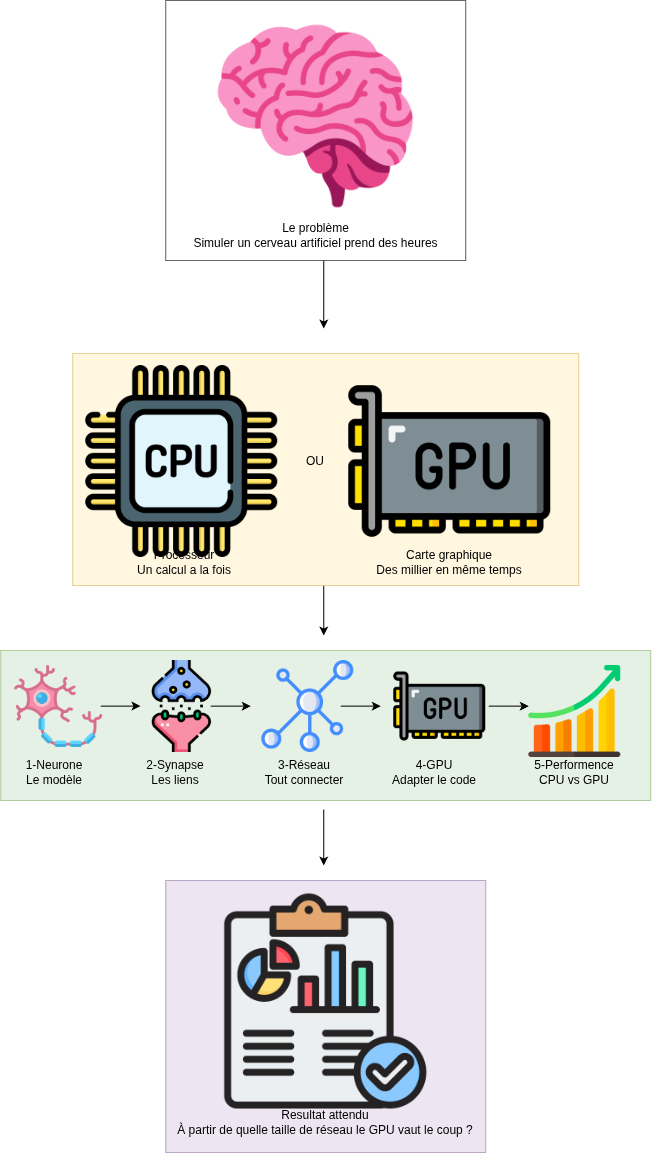
\includegraphics[height=0.92\textheight]{Shema_livrable1.png}
\caption{Carte conceptuelle du projet : qui, quoi, comment, pourquoi, enjeux et contraintes.}
\end{figure}



\part{Livrable 2 : Note de clarification}
\label{part:l2}
\chapter{Objet de la note}

Ce document est le livrable L2 du projet R\&D : la \textbf{note de clarification}. Le livrable L1 a reformulé le sujet et posé la carte conceptuelle, autrement dit \emph{ce qu'est} le sujet. Avant d'entrer dans l'état de l'art et l'analyse fonctionnelle, il reste à préciser \emph{ce que le projet doit produire, pour qui, dans quel cadre et jusqu'où il va} : c'est le rôle de la présente note.

Le cadrage prend en \textbf{entrée} un client porteur de macro-besoins, le laboratoire de M.~Pirog, et un existant, le socle de code \textbf{CPU} fourni. En \textbf{sortie}, il doit donner le contexte et la définition du projet, la vision et les objectifs, les livrables, les étapes clés et le macro-planning, les acteurs et leurs rôles, enfin les contraintes et les risques. Cette note rédige cette synthèse : elle vaut \og contrat \fg{} avec le client et sert de base au \textbf{GO / NO GO} sur la vision commune du projet.

Trois objectifs la guident :
\begin{itemize}
    \item \textbf{écrire noir sur blanc le besoin} du client et des parties prenantes tel que nous l'avons compris, pour que les encadrants le valident ou le corrigent ;
    \item \textbf{délimiter le périmètre} du projet : ce qui est inclus, ce qui est exclu explicitement, et sur quelles hypothèses nous travaillons ;
    \item \textbf{poser des critères de réussite mesurables}, qui guideront l'état de l'art (L3), l'analyse fonctionnelle (L4) et la stratégie de réalisation (L5).
\end{itemize}

Pour la rédiger, nous nous appuyons sur le sujet \og Optimisation de modèles neuronaux à oscillateurs couplés \fg{}, sur le support du projet et sur le socle de code fourni : modèle de \textbf{Hodgkin-Huxley}, \textbf{synapses} et solveur \textbf{CPU} de référence.

Il s'agit aussi d'un document d'\textbf{engagement} : numéroté et daté, il fixe par écrit la vision commune du projet et sera remis à jour au fil des avancées et des clarifications apportées par les encadrants.

\chapter{Contexte et besoin}

\section{Contexte}

Le laboratoire de M.~Antoine Pirog étudie des réseaux de neurones biophysiques par simulation. Le modèle de \textbf{Hodgkin-Huxley} en forme la base : chaque neurone y devient un système d'\textbf{EDO} qui décrit son potentiel membranaire et ses canaux ioniques, et les neurones sont reliés par des modèles biophysiques de \textbf{synapses}, répartis selon la topologie d'un \textbf{connectome}.

La difficulté centrale est identifiée depuis longtemps : le coût d'une simulation augmente avec la taille du réseau, au point de devenir vite rédhibitoire sur \textbf{CPU}. Les réseaux que le laboratoire peut étudier s'en trouvent bornés, et avec eux les questions scientifiques qu'il peut aborder. Junia met à disposition des serveurs à \textbf{GPU} \textbf{RTX~5090} dont la puissance théorique mérite qu'on évalue un portage. Le projet peut aussi aboutir à une autre conclusion : qu'une architecture différente, par exemple le \textbf{FPGA}, performant sur les calculs répétitifs, conviendrait mieux. Cette piste reste ouverte comme alternative au \textbf{GPU}.

\section{Définition du projet et vision}

\textbf{Définition.} Le projet doit mesurer, de façon reproductible, le gain de temps de calcul apporté par un portage \textbf{GPU} de la simulation de réseaux de neurones \textbf{Hodgkin-Huxley} couplés, et déterminer si ce gain suffit à simuler des connectomes nettement plus grands que la référence \textbf{CPU}, sans perdre en fidélité numérique.

\textbf{Vision.} À terme, le laboratoire doit disposer d'un \textbf{environnement de simulation générique} : le modèle neuronal et le connectome se choisissent par configuration, la simulation tourne sur \textbf{CPU} ou sur \textbf{GPU}, et un benchmark documenté dit dans quels cas le \textbf{GPU} se justifie. Une réponse négative aurait la même valeur scientifique : elle épargnerait au laboratoire un investissement inutile.

\section{Besoin exprimé}

Le besoin du laboratoire se formule ainsi :

\begin{quote}
\itshape Le laboratoire a besoin de pouvoir simuler des réseaux de neurones biophysiques de grandes tailles  dans un temps de calcul acceptable, afin d'étudier des connectomes assez grands pour être utiles à la recherche, et de savoir si l'architecture \textbf{GPU} dont il dispose apporte un gain réel face à la référence \textbf{CPU}.
\end{quote}

Deux points précisent ce besoin :
\begin{itemize}
    \item l'objectif n'est pas de passer sur \textbf{GPU} à tout prix, mais de savoir si le \textbf{GPU} se justifie et à quelles conditions : une conclusion négative constituerait, en soi, un résultat ;
    \item les résultats obtenus sur \textbf{GPU} resteront comparables à ceux de la référence \textbf{CPU} : pas d'accélération au prix d'une dérive numérique par rapport au modèle de référence.
\end{itemize}

\section{Données d'entrée}

Le projet démarre avec les éléments suivants, fournis ou imposés :

\begin{itemize}
    \item \textbf{Le sujet} : \og Optimisation de modèles neuronaux à oscillateurs couplés \fg{}.
    \item \textbf{Le socle de code fourni} : modèle de \textbf{Hodgkin-Huxley}, synapses et solveur \textbf{CPU}.
    \item \textbf{Les connectomes} : générés artificiellement avec une structure, rangés dans une matrice de taille $N \times N$ ; aucune donnée biologique réelle n'entre dans le projet.
    \item \textbf{Le benchmark CPU existant} : limité pour l'instant à la topologie en chaîne et à de petites tailles ($N \in \{2, 4, 8, 16\}$), très en dessous des tailles visées ; il servira de point de départ avant d'être étendu.
    \item \textbf{Le matériel} : serveurs Junia à \textbf{GPU RTX~5090}.
    \item \textbf{Le calendrier du projet} : jalons et évaluations imposés (voir la section~\ref{sec:l2-livrables}).
\end{itemize}

\section{Bête à cornes}

La bête à cornes ci-dessous formalise ce besoin : le système rend service au laboratoire, dans le but d'étudier, en un temps de calcul acceptable, des réseaux de neurones assez grands pour la recherche, en agissant sur les modèles de neurones couplés et les connectomes donnés en entrée.

\begin{figure}[!htbp]
\centering
\scalebox{0.8}{%
\begin{tikzpicture}[
    >={Stealth[length=2.4mm,width=1.9mm]},
    ans/.style={
        rectangle, rounded corners=4pt, align=left,
        line width=1pt, inner sep=8pt, font=\footnotesize,
        text=cardink
    },
    qlabel/.style={
        rectangle, rounded corners=3pt, align=center, font=\scriptsize\bfseries,
        inner sep=4pt, text=white
    },
    link/.style={->, line width=1.1pt, draw=cardline, rounded corners=4pt}
]

% =====================================================================
%  Les deux cornes : A QUI | SUR QUOI
% =====================================================================
\node[ans, draw=whyborder, fill=whybg, text width=4.3cm] (QUI) at (-5.3,2.4) {%
    Laboratoire de recherche de M.~Pirog :\\[4pt]
    -- chercheurs en neurosciences computationnelles ;\\[4pt]
    -- encadrants du projet R\&D.};

\node[ans, draw=defiborder, fill=defibg, text width=4.3cm] (MILIEU) at (5.3,2.4) {%
    Les modèles de neurones Hodgkin-Huxley couplés par synapses et les connectomes structurés synthétiques,\\[4pt]
};

\node[qlabel, fill=whyborder, anchor=south west] at ([xshift=4pt]QUI.north west) {À qui rend-il service ?};
\node[qlabel, fill=defiborder, anchor=south west] at ([xshift=4pt]MILIEU.north west) {Sur quoi agit-il ?};

% =====================================================================
%  Le produit au centre
% =====================================================================
\node[ans, draw=hubbg, fill=hubbg, text width=8.6cm, text=white, align=center] (SYS) at (0,-1.8) {%
    {\scriptsize\bfseries LE SYSTÈME}\\[6pt]
    {\small\bfseries Environnement de simulation de réseaux de neurones couplés sur \textbf{GPU}}
};

% =====================================================================
%  Le bas : DANS QUEL BUT
% =====================================================================
\node[ans, draw=whatborder, fill=whatbg, text width=10.6cm, align=center] (BUT) at (0,-6.0) {%
    Étudier des connectomes assez grands pour être utiles à la recherche,\\[4pt]
    dans un temps de calcul acceptable,\\[4pt]
    et savoir si le \textbf{GPU} vaut le coup face au \textbf{CPU}.};

\node[qlabel, fill=whatborder, anchor=south west] at ([xshift=4pt]BUT.north west) {Dans quel but ?};

% =====================================================================
%  Liaisons
% =====================================================================
\draw[link] (QUI.south) -- (SYS.west);
\draw[link] (SYS.east) -- (MILIEU.south);
\draw[link] (SYS.south) -- (BUT.north);

\end{tikzpicture}}%
\caption{Bête à cornes du projet : à qui rend-il service, sur quoi agit-il, dans quel but ?}
\label{fig:bete-l2}
\end{figure}

\chapter{Client et parties prenantes}

\begin{longtable}{|p{4.6cm}|p{10cm}|}
\hline
\textbf{Partie prenante} & \textbf{Rôle} \\ \hline
M.~Antoine Pirog & Client principal, encadrant \\ \hline
M.~Frédéric Chatrie & Encadrant \\ \hline
Laboratoire de recherche & Utilisateur final \\ \hline
Étudiants du projet R\&D & Réalisateurs \\ \hline
\end{longtable}

\chapter{Objectifs}

Les six attentes du sujet deviennent ici des objectifs opérationnels :

\begin{enumerate}
    \item \textbf{Bâtir une référence fiable} : implémenter le modèle de \textbf{Hodgkin-Huxley} avec son terme de couplage synaptique, puis valider sur \textbf{CPU} une implémentation de référence qui servira de vérité terrain.
    \item \textbf{Faire tourner des connectomes structurés} de plus en plus grands : d'abord de petits réseaux de validation, puis des réseaux de plusieurs milliers à dizaines de milliers de neurones.
    \item \textbf{Développer et comparer des stratégies d'optimisation} \textbf{GPU} de la simulation : parallélisation par neurone, gestion des accès mémoire au connectome.
    \item \textbf{Mesurer comment le temps de calcul évolue} avec la taille du connectome, sur \textbf{CPU} comme sur \textbf{GPU}.
    \item \textbf{Livrer un benchmark comparatif} des approches et des stratégies d'optimisation testées.
    \item \textbf{Concevoir un environnement générique} où le modèle neuronal et le connectome se remplacent pour d'autres applications sans réécrire la chaîne de simulation.
\end{enumerate}

\section{Livrables}
\label{sec:l2-livrables}

Les six livrables se font au premier semestre :

\begin{itemize}
    \item \textbf{L1 -- Reformulation du sujet avec schéma expliqué}.
    \item \textbf{L2 -- Note de clarification} (le présent document).
    \item \textbf{L3 -- État de l'art sous forme de benchmark}.
    \item \textbf{L4 -- Analyse fonctionnelle}.
    \item \textbf{L5 -- FAST et schéma synoptique}.
    \item \textbf{Rapport final et soutenance}.
\end{itemize}

Le travail après ces livrables se déroule au second semestre, dans la limite des 100~h de réalisation. Il suit trois phases, chiffrées en durées indicatives :

\begin{itemize}
    \item première phase de développement : environ 2 mois, soit autour de 60~h ;

    \item phase de tests et de benchmark : environ 2 semaines, soit autour de 15~h ;

    \item interprétation des résultats puis deuxième phase de développement : environ 1 mois, soit autour de 25~h.
\end{itemize}

\chapter{Périmètre}

\section{Ce qui est inclus}

\begin{itemize}
    \item Le modèle de \textbf{Hodgkin-Huxley} et le couplage synaptique du socle de code fourni.
    \item Des connectomes artificiels à structure (topologies régulières ou aléatoires), par tailles croissantes.
    \item Un code de référence pour \textbf{CPU}.
    \item Les nombreux documents et ressources existants sur le modèle de \textbf{Hodgkin-Huxley} sur \textbf{CPU}.
\end{itemize}

\section{Ce qui est explicitement exclu}

\begin{itemize}
    \item Toute simulation sur données biologiques réelles (connectomes mesurés) : seuls des connectomes synthétiques sont utilisés.
    \item La modification du modèle biophysique : il ne s'agit pas de chercher un nouveau modèle neuronal, mais d'optimiser la simulation du modèle fourni.
    \item Le temps réel et l'interaction homme-machine pendant la simulation.
\end{itemize}

\chapter{Contraintes, hypothèses et risques}

\section{Contraintes}

\begin{itemize}
    \item \textbf{Temps} : 32~h encadrées au S7 pour les études, puis 100~h au S8 pour la réalisation ; le calendrier du projet impose ses jalons (évaluations du 08/10 et du 22/10).
    \item \textbf{Matériel} : des serveurs Junia à \textbf{RTX~5090} ; la mémoire du \textbf{GPU}, 32~Go de \textbf{VRAM}, borne physiquement la taille des connectomes simulables.
    \item \textbf{Couplage irrégulier} : les connexions du connectome n'ont pas de régularité, les accès mémoire ne sont pas uniformes et une partie du calcul reste séquentielle, les pas de temps s'enchaînant l'un après l'autre ; le parallélisme ne sera donc ni parfait ni simple.
    \item \textbf{Techniques} : des langages dictés par l'existant et par le \textbf{GPU} : socle \textbf{Python} pour la référence, puis \textbf{C/C++/CUDA} ou un framework \textbf{Python} pour l'accélération et la parallélisation.
\end{itemize}

\section{Hypothèses de travail}

\begin{itemize}
    \item Le socle fourni (modèle, synapses, solveur \textbf{CPU}) est juste et peut servir de référence sans revalider en profondeur le modèle biophysique ; le portage \textbf{GPU} se fera dans un langage comme \textbf{C++} ou \textbf{CUDA}.
    \item Les temps mesurés sur les connectomes synthétiques représentent bien ce qu'on obtiendrait sur d'autres connectomes de même structure.
    \item Le benchmark commencera par les pires cas, les connectomes les plus denses (tout-à-tout), puis comparera avec des connectomes creux, plus légers : l'écart entre les deux mesurera l'effet de la densité de connexions sur les performances.
\end{itemize}

\section{Risques}

\begin{longtable}{|p{6.8cm}|p{7.8cm}|}
\hline
\textbf{Risque} & \textbf{Impact} \\ \hline
Mémoire du \textbf{GPU} trop juste pour les plus grands connectomes &
La taille des réseaux mesurables plafonne \\ \hline

Gain exagéré par une référence \textbf{CPU} non optimisée &
Conclusion erronée pour le laboratoire \\ \hline

\end{longtable}

\chapter{Critères de réussite}

\begin{longtable}{|p{5.5cm}|p{9.5cm}|}
\hline
\textbf{Objectif} & \textbf{Critère de réussite mesurable} \\ \hline

Portage \textbf{GPU} valide \textit{ou alternative} &
Les sorties du portage \textbf{GPU} collent à la référence \textbf{CPU} à une tolérance numérique près, définie et justifiée. \\ \hline

Mesures de performance &
Courbes du temps de calcul selon la taille du connectome, sur \textbf{CPU} et \textbf{GPU}, sur une gamme couvrant au moins deux ordres de grandeur. \\ \hline

Benchmark comparatif &
Tableau des stratégies testées avec les mêmes métriques (temps, speedup) et un protocole décrit et reproductible. \\ \hline

Environnement générique &
Le connectome ou le modèle se remplace par configuration, sans toucher au cœur de la chaîne de simulation. \\ \hline

\end{longtable}

\chapter{Suivi et validation de la note}

\section{Décision : GO / NO GO}

La validation de cette note vaut \textbf{GO} : les parties s'accordent sur le besoin, les objectifs, le périmètre et les durées décrits, et le projet se poursuit sur cette base. Un \textbf{GO sous réserve} n'engage la suite qu'une fois les réserves levées ; un \textbf{NO GO} signale un désaccord à lever : la note est alors corrigée et soumise à nouveau, chaque modification étant tracée dans l'historique des versions.

\begin{tabular}{|p{3.4cm}|c|c|c|p{4.4cm}|}
\hline
\textbf{Partie} & \textbf{GO} & \textbf{GO sous réserve} & \textbf{NO GO} & \textbf{Observations} \\ \hline
Équipe projet & $\checkmark$ & $\square$ & $\square$ & \rule{0pt}{0.9cm} \\ \hline
Client (M.~Pirog) & $\checkmark$ & $\square$ & $\square$ & \rule{0pt}{0.9cm} \\ \hline
\end{tabular}

\medskip

Date de la décision : 02/10/2026 {\hrulefill}



\part{Livrable 3 : État de l'art sous forme de benchmark}
\label{part:l3}
\chapter{Introduction}

Ce document est le livrable L3 du projet : l'état de l'art sous forme de benchmark. La note de clarification (L2) a posé le besoin : savoir si les serveurs \textbf{GPU} \textbf{RTX~5090} de Junia permettent de simuler des réseaux de neurones de \textbf{Hodgkin-Huxley} couplés nettement plus grands que sur \textbf{CPU}, dans un temps acceptable et sans dérive numérique. Ce document cherche ce que la littérature dit déjà de cette question, pour préparer nos propres mesures.

Nous avons retenu cinq travaux parus entre 2008 et 2025, cherchés dans des sources reconnues : \textbf{IEEE Xplore}, PubMed Central, ScienceDirect, l'\textbf{ACM} Digital Library et arXiv. Les critères de sélection : simuler des réseaux de neurones (de préférence à conductance, comme Hodgkin-Huxley) ou des systèmes d'\textbf{EDO} sur \textbf{GPU}, avec des mesures de performance publiées. Chacun fait l'objet d'une fiche d'analyse à six questions (chapitre~\ref{chap:l3-fiches}) ; leur synthèse donne le benchmark comparatif du chapitre~\ref{chap:l3-bench}.

D'autres sources complètent cette analyse sans faire l'objet d'une fiche : la fiche technique de la \textbf{RTX~5090}, notre matériel cible \cite{techpowerup} ; une simulation de réseaux fortement connectés sur \textbf{GPU}, notre pire cas \cite{golosio2021} ; la parallélisation sur \textbf{GPU} du solveur des équations d'un neurone multi-compartiments \cite{vooturi2018} ; et la multiplication de matrices creuses sur \textbf{GPU} \cite{bell2009}, la forme sous laquelle notre connectome sera stocké. Toutes sont citées en bibliographie.

\chapter{Fiches d'analyse des articles}
\label{chap:l3-fiches}

\section{Scalable Parallel Programming with CUDA (2008)}

Cet article fondateur, écrit par des ingénieurs \textbf{NVIDIA} et un universitaire \cite{nickolls2008}, explique le modèle de programmation \textbf{CUDA} au moment où les \textbf{CPU} deviennent multicœurs et les \textbf{GPU} massivement parallèles.

\medskip
\begin{tabular}{|p{3.2cm}|p{11.2cm}|}
\hline
\textbf{Pourquoi ?} & Les processeurs grand public gagnent désormais en nombre de cœurs plutôt qu'en fréquence : le matériel devient parallèle, et les logiciels classiques ne le sont pas. Le problème posé : écrire des programmes qui passent à l'échelle quel que soit le nombre de cœurs. \\ \hline
\textbf{Comment ?} & Le modèle \textbf{CUDA} repose sur trois abstractions : une hiérarchie de groupes de fils d'exécution, des mémoires partagées et des barrières de synchronisation. Le programmeur répartit le travail en blocs de fils sans connaître le nombre de cœurs : le matériel s'occupe de l'ordonnancement. \\ \hline
\textbf{Avec quoi ?} & Cartes \textbf{GPU} \textbf{NVIDIA} et kit de développement \textbf{CUDA}, illustrés par des exemples d'applications scientifiques parallèles. \\ \hline
\textbf{Quels résultats ?} & Un même programme \textbf{CUDA} s'exécute sur des \textbf{GPU} de quelques dizaines ou de plusieurs centaines de cœurs sans être réécrit : le parallélisme suit le matériel. \\ \hline
\textbf{Quelles limites ?} & Article de présentation de 2008 : matériel et outils datés, pas de mesure sur des \textbf{EDO} biologiques, et le programmeur travaille toujours à un niveau bas (gestion fine de la mémoire et des fils). \\ \hline
\textbf{Pour notre sujet ?} & C'est le socle conceptuel du projet : paralléliser Hodgkin-Huxley voudra dire répartir les neurones sur des fils d'exécution et organiser la mémoire partagée pour le couplage synaptique. \\ \hline
\end{tabular}

\newpage

\section{GeNN : a code generation framework for accelerated brain simulations (2016)}

GeNN (\emph{GPU-enhanced Neuronal Networks}) est une bibliothèque open source développée à l'université de Sussex pour mettre les \textbf{GPU} à portée des neuroscientifiques \cite{yavuz2016}.

\medskip
\begin{tabular}{|p{3.2cm}|p{11.2cm}|}
\hline
\textbf{Pourquoi ?} & Simuler des réseaux de neurones réalistes est lent, et les accélérateurs \textbf{GPU} restent inaccessibles à ceux qui ne savent pas programmer à bas niveau. \\ \hline
\textbf{Comment ?} & L'utilisateur décrit ses neurones et ses synapses dans une interface de haut niveau ; GeNN génère automatiquement le code \textbf{CUDA} correspondant, sans exiger de connaissances \textbf{GPU} approfondies. \\ \hline
\textbf{Avec quoi ?} & \textbf{GPU} \textbf{NVIDIA} ; bancs d'essai sur plusieurs modèles de réseaux, dont un réseau d'un million de neurones de \textbf{Hodgkin-Huxley} à conductance. \\ \hline
\textbf{Quels résultats ?} & Jusqu'à 200 fois plus rapide qu'un cœur de \textbf{CPU} pour le réseau d'un million de neurones \textbf{Hodgkin-Huxley} ; mais le gain change selon le modèle simulé. \\ \hline
\textbf{Quelles limites ?} & Gain très dépendant du modèle ; comparaison faite contre un seul cœur de \textbf{CPU}, donc une référence faible ; \textbf{NVIDIA} uniquement. \\ \hline
\textbf{Pour notre sujet ?} & Preuve directe qu'un réseau de \textbf{Hodgkin-Huxley} à conductance passe à l'échelle sur \textbf{GPU}, et première forme de l'idée de génération de code que notre projet pourra réutiliser ou comparer à des noyaux écrits à la main. \\ \hline
\end{tabular}

\section{Brian2CUDA : Flexible and Efficient Simulation of Spiking Neural Network Models on GPUs (2022)}

Brian2CUDA ajoute un backend \textbf{GPU} au simulateur Brian2, très utilisé en neurosciences computationnelles \cite{alevi2022}.

\medskip
\begin{tabular}{|p{3.2cm}|p{11.2cm}|}
\hline
\textbf{Pourquoi ?} & Les chercheurs décrivent leurs modèles en \textbf{Python} avec le simulateur Brian2, mais celui-ci n'avait pas de sortie \textbf{GPU} complète : écrire le code bas niveau soi-même demandait un savoir-faire rare. \\ \hline
\textbf{Comment ?} & Le simulateur génère lui-même le code \textbf{CUDA} à partir de la définition du modèle en \textbf{Python} : un volet pour l'intégration numérique des états des neurones, un autre pour la propagation des événements synaptiques. \\ \hline
\textbf{Avec quoi ?} & Code \textbf{CUDA} généré ; comparaisons avec le backend \textbf{CPU} de Brian sur plusieurs types de modèles, y compris neurones et synapses arbitraires et plasticité. \\ \hline
\textbf{Quels résultats ?} & Jusqu'à trois ordres de grandeur d'accélération face au backend \textbf{CPU} de Brian ; seule solution \textbf{GPU} qui couvre toutes les fonctionnalités de Brian2. \\ \hline
\textbf{Quelles limites ?} & Lié au cadre Brian2 : on doit écrire ses modèles dans ce simulateur ; gain variable selon les modèles ; un seul \textbf{GPU}. \\ \hline
\textbf{Pour notre sujet ?} & Démontre qu'on peut accélérer sans écrire de \textbf{CUDA} à la main : le modèle décrit en \textbf{Python} est traduit. Notre socle \textbf{Python}/SciPy pourrait suivre la même voie : compiler les équations plutôt que réécrire le solveur. \\ \hline
\end{tabular}
\newpage
\section{Automated Translation and Accelerated Solving of Differential Equations on Multiple GPU Platforms (2024)}

Cet article, publié dans Computer Methods in Applied Mechanics and Engineering \cite{utkarsh2024}, cherche à résoudre beaucoup d'\textbf{EDO} sur \textbf{GPU} sans écrire de code compliqué, et quel que soit le constructeur de la carte.

\medskip
\begin{tabular}{|p{3.2cm}|p{11.2cm}|}
\hline
\textbf{Pourquoi ?} & Résoudre beaucoup d'\textbf{EDO} sur \textbf{GPU} oblige normalement à écrire du code \textbf{CUDA} à la main, et ce code ne fonctionne que sur les cartes \textbf{NVIDIA}. \\ \hline
\textbf{Comment ?} & Le solveur d'\textbf{EDO} du langage \textbf{Julia} traduit tout seul le code pour la carte : on écrit ses équations comme d'habitude, et elles s'exécutent sur le \textbf{GPU} sans rien changer au modèle. \\ \hline
\textbf{Avec quoi ?} & Des \textbf{GPU} de quatre constructeurs (\textbf{NVIDIA}, AMD, Intel, Apple), et des comparaisons avec du \textbf{CUDA-C++} écrit à la main puis avec \textbf{JAX} et \textbf{PyTorch}. \\ \hline
\textbf{Quels résultats ?} & Aussi rapide que du \textbf{CUDA-C++} optimisé à la main, et 20 à 100 fois plus rapide que la solution de \textbf{JAX} et \textbf{PyTorch}. Le même code tourne sur toutes les cartes testées. \\ \hline
\textbf{Quelles limites ?} & Les \textbf{EDO} de l'article sont indépendantes les unes des autres : pas de synapses ni de connectome, donc pas de couplage irrégulier comme dans notre cas. Et il faut travailler en \textbf{Julia}. \\ \hline
\textbf{Pour notre sujet ?} & Notre réseau est justement un gros système d'\textbf{EDO}. L'article montre qu'on peut éviter d'écrire le \textbf{CUDA} nous-mêmes et ne pas dépendre d'un seul constructeur. Reste à vérifier si ça marche aussi bien quand les équations sont couplées entre elles. \\ \hline
\end{tabular}

\section{SimHH : A Versatile, Multi-GPU Simulator for Extended Hodgkin-Huxley Networks (2025)}

SimHH est le travail le plus récent et le plus proche de notre cas : un simulateur de réseaux de \textbf{Hodgkin-Huxley} étendus, distribué sur des clusters de calcul \cite{engelen2025}.

\medskip
\begin{tabular}{|p{3.2cm}|p{11.2cm}|}
\hline
\textbf{Pourquoi ?} & Les réseaux de \textbf{Hodgkin-Huxley} étendus (multi-compartiments, jonctions communicantes) dépassent ce qu'une seule machine peut simuler en un temps raisonnable. \\ \hline
\textbf{Comment ?} & Répartition de la simulation sur plusieurs nœuds de calcul avec \textbf{MPI} (OpenMPI), avec deux configurations : partager tous les potentiels entre nœuds, ou ne partager que les potentiels utiles ; \textbf{CUDA} et \textbf{NVLink} pour le calcul, les noyaux tournant en parallèle des communications. \\ \hline
\textbf{Avec quoi ?} & Clusters multi-\textbf{GPU} allant jusqu'à 256 nœuds ; modèles étendus dont le noyau inféro-olivaire ; comparaisons avec des \textbf{CPU}, un \textbf{FPGA} et le simulateur \textbf{NEST}. \\ \hline
\textbf{Quels résultats ?} & Réseaux de plus de 10 millions de cellules ; environ 150$\times$ plus rapide qu'un \textbf{CPU} mono-fil, 10$\times$ qu'un \textbf{CPU} à 128 fils, 10$\times$ qu'un \textbf{FPGA}, et 7$\times$ que \textbf{NEST} sur 32 nœuds pour un réseau de 94\,720 neurones à jonctions communicantes. \\ \hline
\textbf{Quelles limites ?} & Exige un cluster de calcul (plusieurs machines reliées) et \textbf{MPI} : une infrastructure bien au-delà d'un serveur universitaire ; la configuration de répartition est délicate à régler. \\ \hline
\textbf{Pour notre sujet ?} & État de l'art le plus proche : \textbf{Hodgkin-Huxley}, comparaisons honnêtes (\textbf{CPU} multi-fils, \textbf{FPGA}, simulateurs) et preuve qu'un seul \textbf{GPU} finit par saturer. Nos mesures se placeront juste avant cette étape multi-\textbf{GPU}. \\ \hline
\end{tabular}

\chapter{Benchmark comparatif}
\label{chap:l3-bench}

Le tableau ci-dessous compare les cinq approches sur les critères de benchmarking. Les gains de performance sont indiqués par rapport à la référence mesurée dans chaque article.

\medskip

{\setlength{\tabcolsep}{3pt}\footnotesize
\begin{tabular}{|p{1.8cm}|p{1.5cm}|p{1.5cm}|p{1.85cm}|p{1.05cm}|p{1.35cm}|p{2.1cm}|p{0.95cm}|}
\hline
\rowcolor{gray!15}
\scriptsize\textbf{Outil} & \scriptsize\textbf{Type} & \scriptsize\textbf{Technicité} & \scriptsize\textbf{Implantation} & \scriptsize\textbf{Coût} & \scriptsize\textbf{Facilité} & \scriptsize\textbf{Gains de performance} & \scriptsize\textbf{Moy.} \\ \hline

CUDA \cite{nickolls2008} & Modèle de programmation \textbf{GPU} &
\cellcolor{bmBest}Très avancé &
\cellcolor{bmBest}Standard en production &
\cellcolor{bmBest}Gratuit &
\cellcolor{bmLow}Complexe &
Sans mesure &
\cellcolor{bmGood}+ \\ \hline

GeNN \cite{yavuz2016} & Génération de code \textbf{CUDA} &
\cellcolor{bmGood}Avancé &
\cellcolor{bmGood}Utilisé en recherche &
\cellcolor{bmBest}Gratuit &
\cellcolor{bmGood}Assez facile &
\cellcolor{bmGood}$\times$200 vs 1 cœur \textbf{CPU} &
\cellcolor{bmGood}+ \\ \hline

Brian2CUDA \cite{alevi2022} & Backend \textbf{GPU} de Brian2 &
\cellcolor{bmMid}Modéré &
\cellcolor{bmMid}Recherche, récent &
\cellcolor{bmBest}Gratuit &
\cellcolor{bmBest}Très facile &
\cellcolor{bmBest}$\times$1000 vs Brian \textbf{CPU} &
\cellcolor{bmGood}+ \\ \hline

Solveur \textbf{Julia} \cite{utkarsh2024} & Solveur d'\textbf{EDO} multi-\textbf{GPU} &
\cellcolor{bmGood}Avancé &
\cellcolor{bmGood}Écosystème actif &
\cellcolor{bmBest}Gratuit &
\cellcolor{bmGood}Facile &
\cellcolor{bmBest}$\times$20--100 vs \textbf{JAX}/\allowbreak\textbf{PyTorch} &
\cellcolor{bmGood}+ \\ \hline

SimHH \cite{engelen2025} & Multi-\textbf{GPU} (\textbf{MPI}) &
\cellcolor{bmBest}Très avancé &
\cellcolor{bmMid}Prototype d'une équipe &
\cellcolor{bmLow}Exige un cluster &
\cellcolor{bmLow}Complexe &
\cellcolor{bmBest}$\times$150 vs \textbf{CPU} mono-fil &
\cellcolor{bmMid}- \\ \hline

\end{tabular}}

\medskip

\begin{tabular}{|p{1.5cm}|p{6cm}|}
\hline
\textbf{Couleur} & \textbf{Signification} \\ \hline
\cellcolor{bmBest} & \textbf{++} Meilleur cas \\ \hline
\cellcolor{bmGood} & \textbf{+} Bon cas \\ \hline
\cellcolor{bmMid} & \textbf{-} Cas plutôt moyen \\ \hline
\cellcolor{bmLow} & \textbf{--} Cas moyen \\ \hline
& Non concerné \\ \hline
\end{tabular}



\part{Livrable 4 : Analyse fonctionnelle}
\label{part:l4}
\chapter{Introduction et expression du besoin}

Ce document est le livrable L4 du projet R\&D : l'\textbf{analyse fonctionnelle}. Le livrable L2 a posé le besoin du laboratoire de M.~Pirog et cadré le projet ; le livrable L3 a montré, par l'état de l'art, les ordres de grandeur que le \textbf{GPU} peut apporter. Ce document fait le passage suivant : il décrit \emph{ce que} le système doit faire, sans préjuger du \emph{comment}, pour préparer les choix techniques du second semestre. Le besoin est d'abord exprimé et validé; les fonctions sont ensuite recensées et représentées par le diagramme pieuvre, puis caractérisées et enfin hiérarchisées pour dégager les fonctions cœur du \textbf{POC}.

Le système étudié est celui de la vision posée en L2 : un \textbf{environnement de simulation de réseaux de neurones couplés sur GPU}. Son besoin, tel que l'a validé la note de clarification, tient en une phrase : \emph{simuler des réseaux de neurones biophysiques de grande taille dans un temps de calcul acceptable, et savoir si le \textbf{GPU} apporte un gain réel face à la référence \textbf{CPU}}.

\section{Bête à cornes}

La bête à cornes qui exprime ce besoin est celle établie lors de la note de clarification, reprise à la figure~\ref{fig:bete-l2}.

\chapter{Fonctions du système}

\section{Liste des fonctions}

Le système doit remplir des fonctions, réparties en trois familles : les fonctions principales (FP), les fonctions secondaires (FS) et les fonctions de contrainte (FC). 

{\small
\begin{longtable}{|p{0.9cm}|p{8.6cm}|p{2.7cm}|}
\hline
\rowcolor{gray!15} \textbf{Code} & \textbf{Fonction} & \textbf{Éléments reliés} \\ \hline
\endhead
\rowcolor{whybg} \textbf{FP1} & Simuler des réseaux de neurones \textbf{Hodgkin-Huxley} couplés par \textbf{synapses}, en calculant l'évolution des potentiels membranaires à chaque pas de temps. & Modèle neuronal, connectome \\ \hline
\rowcolor{whybg} \textbf{FP2} & Accélérer la simulation sur \textbf{GPU}. & Serveurs \textbf{GPU}, référence \textbf{CPU} \\ \hline
\rowcolor{whybg} \textbf{FP3} & Restituer les résultats aux chercheurs (tracés, temps de calcul, erreurs) sous une forme lisible et exploitable. & Chercheur, modèle neuronal \\ \hline
\rowcolor{whatbg} \textbf{FS1} & S'adapter à différentes tailles et topologies de connectomes. & Connectome  \\ \hline
\rowcolor{whatbg} \textbf{FS2} & Adapter les équations du modèle neuronal pour simuler d'autres phénomènes (autres modèles de neurones, variantes des équations) sans réécrire la chaîne de simulation. & Modèle neuronal  \\ \hline
\rowcolor{whatbg} \textbf{FS3} & Garantir des mesures reproductibles : protocole de benchmark documenté, mesures répétées, graines fixées. & Encadrants  \\ \hline
\rowcolor{defibg} \textbf{FC1} & Respecter le modèle de \textbf{Hodgkin-Huxley} et sa méthode de résolution : mêmes équations, même schéma d'intégration que le socle de référence. & Référence \textbf{CPU} \\ \hline
\rowcolor{defibg} \textbf{FC2} & Fonctionner sur le matériel cible : un \textbf{GPU}. & Serveurs \textbf{GPU} \\ \hline
\rowcolor{defibg} \textbf{FC3} & Respecter le temps et le calendrier du projet (32~h d'études au S7, 100~h de réalisation au S8, jalons imposés). & Calendrier \\ \hline
\end{longtable}}

\section{Diagramme pieuvre}

Le système interagit avec plusieurs éléments de son environnement : le chercheur du laboratoire, le modèle neuronal, le connectome, les serveurs GPU, ou encore la référence CPU. Ces interactions sont traduites par des fonctions principales, secondaires et des contraintes, présentées dans le diagramme pieuvre ci-dessous.

\begin{figure}[H]
\centering
\scalebox{0.82}{%
\begin{tikzpicture}[
    milieu/.style={ellipse, draw=cardline, fill=gray!8, line width=1pt, align=center,
        font=\footnotesize\bfseries, text=cardink, inner sep=1pt, minimum height=1.1cm, minimum width=2.9cm},
    fp/.style={line width=1.5pt, draw=whyborder},
    fs/.style={line width=1.5pt, draw=whatborder},
    fc/.style={line width=1.5pt, draw=defiborder},
    lab/.style={font=\scriptsize\bfseries, fill=white, inner sep=1.5pt, rounded corners=2pt}
]
% --- Système : bulle claire, les traits passent par-dessus --------------------
\node[rectangle, rounded corners=12pt, fill=hubrule!35, draw=hubbg, line width=1.4pt,
      minimum width=6.8cm, minimum height=3.4cm] (SYS) at (0,0) {};
\node[align=center, font=\small\bfseries, text=hubbg] at (0,0)
      {Environnement de simulation\\de réseaux de neurones\\couplés sur GPU};

% --- Éléments extérieurs ----------------------------------------------------
\node[milieu] (CH) at (-6.6,3.0) {Chercheur du\\laboratoire};
\node[milieu] (MO) at (-2.2,4.9) {Modèle neuronal\\(Hodgkin-Huxley)};
\node[milieu] (CO) at (6.6,3.0) {Connectome};
\node[milieu] (REF) at (-7.6,-0.4) {Référence CPU\\(socle fourni)};
\node[milieu] (GPU) at (7.6,-0.4) {Serveurs GPU\\Junia (RTX 5090)};
\node[milieu] (CAL) at (-4.2,-4.4) {Calendrier\\du projet};
\node[milieu] (ENC) at (4.2,-4.4) {Encadrants\\(évaluation)};

% --- Fonctions principales : le trait traverse la bulle -----------------------
\draw[fp] (CH.south east) .. controls (-4.0,1.3) and (-3.5,0.6) .. node[lab, text=whyborder, pos=0.3]{FP3} (-2.6,0.75)
          .. controls (-1.9,0.9) and (-2.1,3.0) .. (MO.south west);
\draw[fp] (MO.south east) .. controls (-0.7,2.8) and (0.3,0.9) .. node[lab, text=whyborder, pos=0.3]{FP1} (1.4,0.9)
          .. controls (2.6,0.9) and (4.6,1.9) .. (CO.south west);
\draw[fp] (REF.east) .. controls (-4.6,-0.6) and (-2.6,-1.05) .. node[lab, text=whyborder, pos=0.25]{FP2} (0,-1.05)
          .. controls (2.6,-1.05) and (4.6,-0.6) .. (GPU.west);

% --- Fonctions secondaires : le trait s'arrête dans la bulle -------------------
\draw[fs] (MO.south) .. controls (-1.8,2.6) and (-1.0,1.7) .. node[lab, text=whatborder, pos=0.3]{FS2} (-0.9,1.05);
\fill[whatborder] (-0.9,1.05) circle (2.2pt);
\draw[fs] (CO.south) .. controls (6.2,1.0) and (4.0,0.5) .. node[lab, text=whatborder, pos=0.3]{FS1} (2.6,0.45);
\fill[whatborder] (2.6,0.45) circle (2.2pt);

% --- Fonctions contraintes -----------------------------------------------------
\draw[fc] (REF.north east) .. controls (-5.0,0.7) and (-3.8,0.2) .. node[lab, text=defiborder, pos=0.3]{FC1} (-2.9,0.1);
\fill[defiborder] (-2.9,0.1) circle (2.2pt);
\draw[fc] (GPU.north west) .. controls (5.0,0.5) and (3.8,-0.35) .. node[lab, text=defiborder, pos=0.3]{FC2} (2.9,-0.35);
\fill[defiborder] (2.9,-0.35) circle (2.2pt);
\draw[fc] (CAL.north) .. controls (-3.6,-2.6) and (-2.2,-1.4) .. node[lab, text=defiborder, pos=0.3]{FC3} (-1.4,-1.38);
\fill[defiborder] (-1.4,-1.38) circle (2.2pt);
\draw[fs] (ENC.north) .. controls (3.6,-2.6) and (2.2,-1.4) .. node[lab, text=whatborder, pos=0.3]{FS3} (1.4,-1.38);
\fill[whatborder] (1.4,-1.38) circle (2.2pt);

% --- Légende ---------------------------------------------------------------
\node[draw=cardline, rounded corners=3pt, fill=white, align=left, font=\scriptsize,
      inner sep=4pt, anchor=north east] at (9.1,5.6) {%
    \tikz\draw[fp] (0,0)--(0.6,0); \ Fonction principale (FP)\\[2pt]
    \tikz\draw[fs] (0,0)--(0.6,0); \ Fonction secondaire (FS)\\[2pt]
    \tikz\draw[fc] (0,0)--(0.6,0); \ Fonction contrainte (FC)};
\end{tikzpicture}}%
\caption{Diagramme pieuvre : les fonctions principales traversent le système pour relier deux éléments extérieurs ; les autres s'arrêtent dans le système.}
\label{fig:pieuvre}
\end{figure}

\chapter{Caractérisation des fonctions}

\section{Méthode}

Chaque fonction est caractérisée par un ou plusieurs \textbf{critères}, un \textbf{niveau} visé pour chacun, une \textbf{tolérance} et une \textbf{flexibilité}. Les classes de flexibilité sont celles du cahier des charges fonctionnel : \textbf{F0} impérative (limite physique ou cadre imposé), \textbf{F1} peu négociable, \textbf{F2} négociable (un résultat en dessous du niveau reste exploitable) et \textbf{F3} très négociable.

\section{Tableau de caractérisation}

Les lignes sont colorées selon la famille de la fonction et les fonctions cœur du \textbf{POC} sont repérées par une étoile (*).

{\small
\setlength{\tabcolsep}{3.5pt}
\begin{longtable}{|p{1.0cm}|p{4.6cm}|p{4.3cm}|p{3.4cm}|p{0.8cm}|}
\hline
\rowcolor{gray!15}
\textbf{Fct.} & \textbf{Critère} & \textbf{Niveau} & \textbf{Tolérance} & \textbf{Flex.} \\ \hline
\endfirsthead
\hline
\rowcolor{gray!15}
\textbf{Fct.} & \textbf{Critère} & \textbf{Niveau} & \textbf{Tolérance} & \textbf{Flex.} \\ \hline
\endhead

\rowcolor{whybg} \textbf{FP1*} & Taille du réseau simulé & $10^3$ neurones & Quelques centaines (100) & F1 \\ \hline
\rowcolor{whybg} & Modèle simulé & Neurone de \textbf{Hodgkin-Huxley} et \textbf{synapse} du socle fourni & Aucune & F0 \\ \hline
\rowcolor{whybg} \textbf{FP2*} & \textbf{Speedup} face à la référence \textbf{CPU} du socle & $\geq 10$ (pour réseau de taille importante) & $> 1$ (un gain nul reste un résultat) & F2 \\ \hline
\rowcolor{whybg} & \textbf{Speedup} face à une référence \textbf{CPU} optimisée (multi-cœur) & Mesuré face au socle seul, limite signalée & Aucune & F1 \\ \hline
\rowcolor{whybg} & Gamme de tailles $N$ et seuil du \textbf{GPU} & Taille à partir de laquelle le \textbf{GPU} devient plus rapide, identifiée pour chaque topologie & Identifiée pour au moins une topologie & F1 \\ \hline
\rowcolor{whybg} \textbf{FP3} & Résultats restitués & Tracés, temps de calcul, erreurs, fichiers lisibles par \textbf{Python} (NumPy, CSV) & Tracés et temps de calcul seuls & F1 \\ \hline
\rowcolor{whybg} & Format des fichiers & Lisible en \textbf{Python} (NumPy, CSV) & Tout format ouvert & F2 \\ \hline
\rowcolor{whatbg} \textbf{FS1*} & Topologies de connectome & Chaîne, tout-à-tout, aléatoire, connectome creux & Chaîne et tout-à-tout suffisent & F1 \\ \hline
\rowcolor{whatbg} \textbf{FS2} & Changement d'équations & Par configuration, sans modifier le moteur & Modification d'un seul fichier ; second modèle si le temps le permet & F1 \\ \hline
\rowcolor{whatbg} \textbf{FS3} & Optimisation du temps et protocole & Calcul et transferts mémoire séparés ; protocole de benchmark écrit dans le rapport & Temps de calcul uniquement & F1 \\ \hline
\rowcolor{defibg} \textbf{FC1*} & Équations et schéma d'intégration & Identiques au socle de référence & Aucune & F0 \\ \hline
\rowcolor{defibg} & Précision des calculs & Double précision (FP64), comme la référence & Simple précision (FP32) si les tracés restent superposés à la référence & F2 \\ \hline
\rowcolor{defibg} \textbf{FC2*} & Matériel et mémoire & \textbf{RTX~5090} $32$~Go de \textbf{VRAM} & Aucune & F0 \\ \hline
\rowcolor{defibg} \textbf{FC3} & Volume horaire et jalons & 32~h au S7 ; 100~h au S8 (60~h de développement, 15~h de tests, 25~h d'analyse) ; jalons respectés & Aucune & F0 \\ \hline
\end{longtable}}

\medskip
\noindent{\small\textbf{Légende.}~%
\tikz\fill[whybg, draw=whyborder, line width=0.5pt] (0,0) rectangle (0.28,0.14);~fonction principale (FP) \quad
\tikz\fill[whatbg, draw=whatborder, line width=0.5pt] (0,0) rectangle (0.28,0.14);~fonction secondaire (FS) \quad
\tikz\fill[defibg, draw=defiborder, line width=0.5pt] (0,0) rectangle (0.28,0.14);~fonction contrainte (FC) \quad
*~: fonction cœur du \textbf{POC}.}

\chapter{Hiérarchisation et fonctions cœur du POC}

\section{Méthode du tri croisé}

Les fonctions sont comparées deux à deux : chaque case de la matrice indique la fonction la plus importante pour le service rendu au laboratoire, et l'écart d'importance va de \textbf{0} (égalité, aucun point) à \textbf{1} (un peu plus), \textbf{2} (plus) et \textbf{3} (beaucoup plus). 

\begin{table}[H]
\centering
{\small
\setlength{\tabcolsep}{3pt}
\renewcommand{\arraystretch}{1.3}
\begin{tabular}{|c|c|c|c|c|c|c|c|c|}
\hline
\cellcolor{gray!15} & \cellcolor{whybg}\textbf{FP2} & \cellcolor{whybg}\textbf{FP3} & \cellcolor{whatbg}\textbf{FS1} & \cellcolor{whatbg}\textbf{FS2} & \cellcolor{whatbg}\textbf{FS3} & \cellcolor{defibg}\textbf{FC1} & \cellcolor{defibg}\textbf{FC2} & \cellcolor{defibg}\textbf{FC3} \\ \hline
\cellcolor{whybg}\textbf{FP1} & \cellcolor{whybg}FP1(1) & \cellcolor{whybg}FP1(2) & \cellcolor{whybg}FP1(2) & \cellcolor{whybg}FP1(3) & \cellcolor{whybg}FP1(2) & \cellcolor{whybg}FP1(1) & \cellcolor{whybg}FP1(1) & \cellcolor{whybg}FP1(2) \\ \hline
\cellcolor{whybg}\textbf{FP2} & \cellcolor{gray!35} & \cellcolor{whybg}FP2(2) & \cellcolor{whybg}FP2(1) & \cellcolor{whybg}FP2(3) & \cellcolor{whybg}FP2(1) & \cellcolor{gray!10}0 & \cellcolor{whybg}FP2(1) & \cellcolor{whybg}FP2(2) \\ \hline
\cellcolor{whybg}\textbf{FP3} & \cellcolor{gray!35} & \cellcolor{gray!35} & \cellcolor{gray!10}0 & \cellcolor{whybg}FP3(2) & \cellcolor{gray!10}0 & \cellcolor{defibg}FC1(1) & \cellcolor{gray!10}0 & \cellcolor{whybg}FP3(1) \\ \hline
\cellcolor{whatbg}\textbf{FS1} & \cellcolor{gray!35} & \cellcolor{gray!35} & \cellcolor{gray!35} & \cellcolor{whatbg}FS1(2) & \cellcolor{whatbg}FS1(1) & \cellcolor{defibg}FC1(1) & \cellcolor{gray!10}0 & \cellcolor{whatbg}FS1(2) \\ \hline
\cellcolor{whatbg}\textbf{FS2} & \cellcolor{gray!35} & \cellcolor{gray!35} & \cellcolor{gray!35} & \cellcolor{gray!35} & \cellcolor{whatbg}FS3(1) & \cellcolor{defibg}FC1(3) & \cellcolor{defibg}FC2(2) & \cellcolor{defibg}FC3(1) \\ \hline
\cellcolor{whatbg}\textbf{FS3} & \cellcolor{gray!35} & \cellcolor{gray!35} & \cellcolor{gray!35} & \cellcolor{gray!35} & \cellcolor{gray!35} & \cellcolor{defibg}FC1(1) & \cellcolor{defibg}FC2(1) & \cellcolor{whatbg}FS3(1) \\ \hline
\cellcolor{defibg}\textbf{FC1} & \cellcolor{gray!35} & \cellcolor{gray!35} & \cellcolor{gray!35} & \cellcolor{gray!35} & \cellcolor{gray!35} & \cellcolor{gray!35} & \cellcolor{defibg}FC1(1) & \cellcolor{defibg}FC1(2) \\ \hline
\cellcolor{defibg}\textbf{FC2} & \cellcolor{gray!35} & \cellcolor{gray!35} & \cellcolor{gray!35} & \cellcolor{gray!35} & \cellcolor{gray!35} & \cellcolor{gray!35} & \cellcolor{gray!35} & \cellcolor{defibg}FC2(1) \\ \hline
\cellcolor{defibg}\textbf{FC3} & \cellcolor{gray!35} & \cellcolor{gray!35} & \cellcolor{gray!35} & \cellcolor{gray!35} & \cellcolor{gray!35} & \cellcolor{gray!35} & \cellcolor{gray!35} & \cellcolor{gray!35} \\ \hline
\end{tabular}}
\caption{Matrice du tri croisé (36 comparaisons).}
\label{tab:tri}
\end{table}

\section{Résultats}

\begin{table}[H]
\centering
{\small
\begin{tabular}{|c|c|c|p{7.6cm}|}
\hline
\rowcolor{gray!15} \textbf{Fonction} & \textbf{Points} & \textbf{Poids} & \textbf{Intitulé} \\ \hline
\textbf{FP1} & \cellcolor{resVert} 14 & \cellcolor{resVert} 29,2\,\% & Simuler des réseaux \textbf{Hodgkin-Huxley} couplés par \textbf{synapses} \\ \hline
\textbf{FP2} & \cellcolor{resVert} 10 & \cellcolor{resVert} 20,8\,\% & Accélérer la simulation sur \textbf{GPU} \\ \hline
\textbf{FC1} & \cellcolor{resJaune} 9 & \cellcolor{resJaune} 18,8\,\% & Respecter le modèle et le schéma d'intégration du socle \\ \hline
\textbf{FS1} & \cellcolor{resJaune} 5 & \cellcolor{resJaune} 10,4\,\% & S'adapter à différentes tailles et topologies de connectomes \\ \hline
\textbf{FC2} & \cellcolor{resOrange} 4 & \cellcolor{resOrange} 8,3\,\% & Fonctionner sur le matériel cible (\textbf{GPU}) \\ \hline
\textbf{FP3} & \cellcolor{resOrange} 3 & \cellcolor{resOrange} 6,3\,\% & Restituer les résultats aux chercheurs \\ \hline
\textbf{FS3} & \cellcolor{resRougeC} 2 & \cellcolor{resRougeC} 4,2\,\% & Garantir des mesures reproductibles \\ \hline
\textbf{FC3} & \cellcolor{resRougeC} 1 & \cellcolor{resRougeC} 2,0\,\% & Respecter le temps et le calendrier du projet \\ \hline
\textbf{FS2} & \cellcolor{resRouge} 0 & \cellcolor{resRouge} 0,0\,\% & Adapter les équations sans réécrire la chaîne de simulation \\ \hline
\textbf{Total} & 48 & 100\,\% & \\ \hline
\end{tabular}}
\caption{Hiérarchisation des fonctions, par poids décroissant ; la couleur va du vert (poids fort) au rouge (poids nul).}
\label{tab:prio}
\end{table}

\begin{figure}[H]
\centering
\begin{tikzpicture}[x=0.6cm, y=0.5cm]
    \foreach \f/\p/\c [count=\i] in {FP1/14/1, FP2/10/1, FC1/9/1, FS1/5/1, FC2/4/1, FP3/3/0, FS3/2/0, FC3/1/0, FS2/0/0} {
        \pgfmathsetmacro{\yy}{-\i}
        \node[anchor=east, font=\footnotesize\bfseries, text=cardink] at (-0.3,\yy) {\f};
        \ifnum\c=1
            \fill[bmMid, draw=pocborder, line width=0.8pt] (0,\yy-0.32) rectangle (\p,\yy+0.32);
        \else
            \fill[gray!25, draw=gray!60, line width=0.8pt] (0,\yy-0.32) rectangle (\p,\yy+0.32);
        \fi
        \node[anchor=west, font=\scriptsize, text=cardink] at (\p+0.2,\yy) {\p~pts};
    }
    \draw[cardline, line width=0.8pt] (0,-0.4) -- (0,-9.6);
    \draw[defiborder, dashed, line width=1.1pt] (-1.6,-5.5) -- (19,-5.5);
    \node[anchor=south east, font=\scriptsize\itshape, text=defiborder] at (19,-5.45) {seuil du POC};
\end{tikzpicture}
\caption{Poids des fonctions issus du tri croisé.}
\label{fig:barres}
\end{figure}

\chapter{Conclusion et perspectives}

Ce livrable fait le point sur ce que le système doit faire pour répondre au besoin du laboratoire de M.~Pirog : simuler de grands réseaux de neurones dans un temps raisonnable, et savoir si le \textbf{GPU} est vraiment plus rapide que le \textbf{CPU}. Le besoin a d'abord été rappelé avec la bête à cornes, puis traduit en fonctions principales, secondaires et de contrainte, reliées aux éléments extérieurs dans le diagramme pieuvre.

Chaque fonction a ensuite été décrite précisément : ce qui est attendu (le critère), jusqu'où (le niveau), et la marge de négociation (la flexibilité). Ce travail fixe des objectifs clairs et chiffrés pour la suite du projet, comme la taille des réseaux visés ou le gain de temps attendu.

Enfin, le tri croisé a permis de classer les fonctions par importance. Les cinq premières -- FP1, FP2, FC1, FS1 et FC2 -- forment les fonctions cœur du \textbf{POC} : elles totalisent \textbf{87,5\,\%} des points, et ce sont elles qui permettront de répondre à la question du projet. Les autres fonctions ne sont pas abandonnées : elles seront traitées plus tard, si le temps du semestre 8 le permet.



\part{Livrable 5 : Rapport de conception}
\label{part:l5}
\chapter{Diagrammes FAST}

Le diagramme \textbf{FAST} se lit de gauche à droite avec la question \og \emph{comment} ? \fg{} ; dans l'autre sens, la même chaîne répond à \og \emph{pourquoi} ? \fg. Chaque sous-fonction est reliée, par une flèche pointillée, à la solution technique (en jaune) qui la réalise. Dans tout le document, $W$ désigne la matrice de connexions du réseau.

\noindent{\small\textbf{Légende.}~%
\tikz\fill[whybg, draw=whyborder, line width=0.5pt] (0,0) rectangle (0.26,0.13);~fonction \quad
\tikz\fill[gray!8, draw=cardline, line width=0.5pt] (0,0) rectangle (0.26,0.13);~sous-fonction \quad
\tikz\fill[bmMid, draw=pocborder, line width=0.5pt] (0,0) rectangle (0.26,0.13);~solution technique.}


\begin{figure}[H]
\centering
\scalebox{0.75}{%
\begin{tikzpicture}[fast]
% Colonnes : fonction (x=0), bus vertical (x=2.4), sous-fonctions (x=6.6), solutions (x=12.6)
\def\xbus{2.4}
\node[fct] (FP1) at (0,0) {FP1\\[2pt]Simuler des réseaux\\Hodgkin-Huxley\\couplés par synapses};

\node[sous] (S1) at (6.6, 3.6) {Décrire le réseau à simuler};
\node[sous] (S2) at (6.6, 1.2) {Faire communiquer les neurones entre eux};
\node[sous] (S3) at (6.6,-1.2) {Faire évoluer le potentiel de chaque neurone};
\node[sous] (S4) at (6.6,-3.6) {Enchaîner les pas de temps jusqu'à la durée};

\node[sol] (T1) at (12.6, 3.6) {Générateur de connectome :\\taille $N$, chaîne,\\tout-à-tout, aléatoire (FS1)\\(\textit{conf.json} pour description du réseau\\Python pour générer la matrice $W$)};
\node[sol] (T2) at (12.6, 1.2) {Chaque neurone intègre\\les messages de ses voisins, selon $W$};
\node[sol] (T3) at (12.6,-1.2) {Résolution Hodgkin-Huxley,\\équations du socle (FC1)};
\node[sol] (T4) at (12.6,-3.6) {Boucle de simulation,\\pas de temps du socle};

\node[font=\scriptsize\itshape, text=cardink] at (6.6,5.0) {Comment ? $\rightarrow$ \quad $\leftarrow$ Pourquoi ?};

% Arborescence orthogonale : tronc commun puis une branche par sous-fonction
\draw[tronc] (FP1.east) -- (\xbus,0);
\draw[tronc] (\xbus,3.6) -- (\xbus,-3.6);
\node[noeud] at (\xbus,0) {};
\foreach \i in {1,...,4}{
    \draw[lien] (\xbus,0 |- S\i.west) -- node[cmt]{Comment ?} (S\i.west);
    \draw[real] (S\i.east) -- (T\i.west);
}
\end{tikzpicture}}%
\caption{FAST de FP1 : le réseau est décrit par le générateur de connectome (FS1), puis simulé pas à pas -- communication entre les neurones, mise à jour Hodgkin-Huxley (FC1) -- jusqu'à la durée choisie.}
\label{fig:fast-fp1}
\end{figure}

\begin{figure}[H]
\centering
\scalebox{0.75}{%
\begin{tikzpicture}[fast]
\def\xbus{2.4}
\node[fct] (FP2) at (0,0) {FP2\\[2pt]Accélérer la\\simulation\\sur GPU};

\node[sous] (S1) at (6.6, 2.4) {Répartir les neurones sur les c\oe urs};
\node[sous] (S2) at (6.6, 0)   {Garder les données sur la carte};
\node[sous] (S3) at (6.6,-2.4) {Piloter la carte sans la ralentir};

\node[sol] (T1) at (12.6, 2.4) {Un fil de calcul par neurone};
\node[sol] (T2) at (12.6, 0)   {VRAM résidente,\\transferts début et fin (FC2)};
\node[sol] (T3) at (12.6,-2.4) {Orchestrateur CPU (Python) :\\lance les calculs à chaque pas};

\node[font=\scriptsize\itshape, text=cardink] at (6.6,3.8) {Comment ? $\rightarrow$ \quad $\leftarrow$ Pourquoi ?};

\draw[tronc] (FP2.east) -- (\xbus,0);
\draw[tronc] (\xbus,2.4) -- (\xbus,-2.4);
\node[noeud] at (\xbus,0) {};
\foreach \i in {1,...,3}{
    \draw[lien] (\xbus,0 |- S\i.west) -- node[cmt]{Comment ?} (S\i.west);
    \draw[real] (S\i.east) -- (T\i.west);
}
\end{tikzpicture}}%
\caption{FAST de FP2 : les neurones sont répartis sur les c\oe urs, les données restent en VRAM (FC2) et l'orchestrateur lance les calculs à chaque pas.}
\label{fig:fast-fp2}
\end{figure}

\chapter{Schéma synoptique}

\begin{figure}[H]
\centering
\scalebox{0.74}{%
\begin{tikzpicture}[
    >={Stealth[length=2.4mm,width=1.9mm]},
    gbloc/.style={rectangle, rounded corners=5pt, draw=cardline, fill=gray!8, line width=0.9pt,
        align=center, font=\footnotesize\bfseries, text=cardink, inner sep=6pt},
    vrbox/.style={rectangle, rounded corners=5pt, draw=whyborder, fill=whybg, line width=1.1pt,
        align=center, font=\footnotesize\bfseries, text=cardink, inner sep=6pt},
    ent/.style={rectangle, rounded corners=5pt, line width=1pt, align=center,
        font=\footnotesize\bfseries, text=white, inner sep=6pt},
    flux/.style={->, line width=1.1pt, draw=cardline},
    io/.style={<->, line width=1pt, draw=cardline},
    cmd/.style={->, line width=1.1pt, draw=defiborder, dashed},
    flab/.style={font=\scriptsize, text=cardink, fill=white, inner sep=1.5pt, rounded corners=2pt}
]
% Trois colonnes alignées : gauche (x=-5), centre (x=0), droite (x=5)
% --- Rangée du haut -------------------------------------------------------
\node[ent, fill=hubbg, text width=3.6cm, minimum height=1.5cm] (CONF) at (-5,12.0)
    {Configuration\\[-1pt]{\scriptsize modèle, $N$, topologie,\\$dt$, durée, graine}};

\node[gbloc, text width=3.6cm, minimum height=1.5cm] (GEN) at (0,12.0)
    {Générateur de connectome\\[-1pt]{\scriptsize matrice $N \times N$}};

\node[gbloc, text width=3.6cm, minimum height=1.5cm] (REF) at (5,12.0)
    {Référence CPU\\[-1pt]{\scriptsize et temps CPU}};

% --- Milieu : hôte CPU ---------------------------------------------------
\node[gbloc, text width=4.6cm] (ORCH) at (-5,7.8)
    {Orchestrateur de simulation\\[-1pt]{\scriptsize hôte CPU, Python\\-- charge la config et le connectome\\-- lance les calculs\\-- récupère les sorties}};

\node[gbloc, text width=4.6cm] (VALID) at (5,7.3)
    {Validation et mesure\\[-1pt]{\scriptsize -- écart sur $V(t)$\\-- speedup $= t_{CPU} / t_{GPU}$}};

\node[gbloc, text width=4.6cm] (RES) at (5,3.9)
    {Restitution\\[-1pt]{\scriptsize -- fichiers CSV / NumPy, tracés\\-- courbes de temps et speedup}};

% --- Zone GPU --------------------------------------------------------------
\node[vrbox, text width=4.4cm, minimum height=5.4cm] (VRAM) at (-5,-1.6)
    {Mémoire VRAM (résidente)\\[-1pt]{\scriptsize -- états des neurones $V, m, h, n$\\-- connectome dense ou CSR\\-- courants et sorties}};

\node[gbloc, text width=4.4cm, minimum height=1.5cm] (N1) at (4.4,0.1)
    {Courants synaptiques\\[-1pt]{\scriptsize chaque neurone additionne\\ses entrées, selon le connectome}};

\node[gbloc, text width=4.4cm, minimum height=1.5cm] (N2) at (4.4,-3.3)
    {Mise à jour des neurones\\[-1pt]{\scriptsize Hodgkin-Huxley, un fil par neurone}};

\node[font=\footnotesize\bfseries, text=hubbg] (GPUT) at (0,1.8)
    {GPU NVIDIA \textbf{RTX 5090} --- 32~Go de \textbf{VRAM}};

\begin{scope}[on background layer]
\node[rectangle, rounded corners=8pt, draw=hubbg, fill=hubrule!18, line width=1.2pt,
      inner xsep=0.5cm, inner ysep=0.35cm, fit=(VRAM)(N1)(N2)(GPUT)] (GPUB) {};
\end{scope}

% --- Encadrement Epreuvage : reference CPU + validation ---------------------
\begin{scope}[on background layer]
\node[rectangle, rounded corners=8pt, dashed, draw=cardline, line width=1.1pt,
      inner xsep=0.25cm, inner ysep=0.6cm, fit=(REF)(VALID)] (EPR) {};
\end{scope}
\node[anchor=south, font=\scriptsize\bfseries, text=cardink, fill=white, inner sep=2pt]
      at (EPR.north) {Epreuvage};

% --- Flux (tous orthogonaux, aucun croisement) ----------------------------
\draw[flux] (CONF.south) -- node[flab]{configuration} (ORCH.north);
\draw[flux] (GEN.south) |- node[flab, pos=0.3]{matrice $W$} ([yshift=5mm]ORCH.east);
\draw[flux] (REF.south) -- node[flab]{sorties et temps CPU} (VALID.north);
\draw[flux, rounded corners=6pt] (ORCH.east) -- (-1.5,7.8) -- (-1.5,6.35) -- (5,6.35)
    -- node[flab, pos=0.5]{sorties et temps GPU} (RES.north);
\draw[cmd] (ORCH.south) -- node[flab, text=defiborder, pos=0.3]{lancement des calculs} (ORCH.south |- GPUB.north);
\draw[flux] (GPUB.north -| -7.0,0) -- node[flab, pos=0.38]{retour des sorties} (ORCH.south -| -7.0,0);

\draw[io] (VRAM.east |- N1.west) -- node[flab]{lit / écrit} (N1.west);
\draw[io] (VRAM.east |- N2.west) -- node[flab]{lit / écrit} (N2.west);
\draw[flux] (N1.south) -- node[flab]{pas suivant} (N2.north);

% --- Légende --------------------------------------------------------------
\node[draw=cardline, rounded corners=3pt, fill=white, align=left, font=\scriptsize,
      inner sep=4pt, below=0.5cm of GPUB] {%
    \tikz\draw[flux] (0,0)--(0.55,0); \ flux d'information \quad
    \tikz\draw[cmd] (0,0)--(0.55,0); \ commande \quad
    \tikz\fill[whybg, draw=whyborder, line width=0.5pt] (0,0) rectangle (0.28,0.16); \ données gardées sur la carte};
\end{tikzpicture}}%
\caption{Schéma synoptique du POC : l'orchestrateur sur CPU pilote la carte GPU ; la référence CPU et les sorties GPU sont comparées puis restituées.}
\label{fig:syno}
\end{figure}

L'orchestrateur, sur le \textbf{CPU} hôte, charge la configuration et le connectome, lance les calculs à chaque pas et récupère les sorties ; pendant ce temps, toute la simulation vit dans la \textbf{VRAM} de la carte, sans transfert en cours de calcul. Les fonctions cœur se repèrent bloc par bloc : FP1 dans les deux calculs de la carte (courants synaptiques et \textbf{Hodgkin-Huxley}), FP2 dans ces calculs et la mesure du \textbf{speedup}, FC1 dans la validation, FS1 dans le générateur et le stockage dense ou \textbf{CSR}, FC2 dans la carte visée (\textbf{RTX~5090}, 32~Go de \textbf{VRAM}).



\begin{thebibliography}{9}
\addcontentsline{toc}{chapter}{Bibliographie}

\bibitem{nickolls2008} J.~Nickolls, I.~Buck, M.~Garland, K.~Skadron, \og Scalable Parallel Programming with CUDA \fg, \emph{ACM Queue}, vol.~6, n\textsuperscript{o}~2, p.~24--32, mars 2008. \href{https://doi.org/10.1145/1365490.1365500}{DOI : 10.1145/1365490.1365500}.

\bibitem{yavuz2016} E.~Yavuz, J.~Turner, T.~Nowotny, \og GeNN : a code generation framework for accelerated brain simulations \fg, \emph{Scientific Reports}, vol.~6, article 18854, 2016. \href{https://doi.org/10.1038/srep18854}{DOI : 10.1038/srep18854}.

\bibitem{alevi2022} D.~Alevi, M.~Stimberg, H.~Sprekeler, K.~Obermayer, M.~Augustin, \og Brian2CUDA : Flexible and Efficient Simulation of Spiking Neural Network Models on GPUs \fg, \emph{Frontiers in Neuroinformatics}, vol.~16, article 883700, 2022. \href{https://doi.org/10.3389/fninf.2022.883700}{DOI : 10.3389/fninf.2022.883700}.

\bibitem{utkarsh2024} U.~Utkarsh, V.~Churavy, Y.~Ma, T.~Besard, P.~Srisuma, T.~Gymnich, A.~R.~Gerlach, A.~Edelman, G.~Barbastathis, R.~D.~Braatz, C.~Rackauckas, \og Automated Translation and Accelerated Solving of Differential Equations on Multiple GPU Platforms \fg, \emph{Computer Methods in Applied Mechanics and Engineering}, vol.~419, 2024. \href{https://doi.org/10.1016/j.cma.2023.116591}{DOI : 10.1016/j.cma.2023.116591}. Prépublication : \href{https://arxiv.org/abs/2304.06835}{arXiv:2304.06835}.

\bibitem{engelen2025} M.~C.~W.~Engelen, J.-H.~L.~F.~Betting, C.~Strydis, \og SimHH : A Versatile, Multi-GPU Simulator for Extended Hodgkin-Huxley Networks \fg, \emph{IEEE Access}, vol.~13, 2025. \href{https://doi.org/10.1109/ACCESS.2025.3550444}{DOI : 10.1109/ACCESS.2025.3550444}.

\bibitem{golosio2021} B.~Golosio, G.~Tiddia, C.~De~Luca, E.~Pastorelli, F.~Simula, P.~S.~Paolucci, \og Fast Simulations of Highly-Connected Spiking Cortical Models Using GPUs \fg, \emph{Frontiers in Computational Neuroscience}, vol.~15, article 627620, 2021. \href{https://doi.org/10.3389/fncom.2021.627620}{DOI : 10.3389/fncom.2021.627620}.

\bibitem{vooturi2018} D.~T.~Vooturi, K.~Kothapalli, U.~S.~Bhalla, \og Parallelizing Hines Matrix Solver in Neuron Simulations on GPU \fg, \emph{2017 IEEE 24th International Conference on High Performance Computing (HiPC)}, p.~388--397, 2018. \href{https://doi.org/10.1109/HiPC.2017.00051}{DOI : 10.1109/HiPC.2017.00051}.

\bibitem{bell2009} N.~Bell, M.~Garland, \og Implementing sparse matrix-vector multiplication on throughput-oriented processors \fg, \emph{Proceedings of the Conference on High Performance Computing, Networking, Storage and Analysis (SC'09)}, ACM, 2009. \href{https://doi.org/10.1145/1654059.1654078}{DOI : 10.1145/1654059.1654078}.

\bibitem{techpowerup} \og NVIDIA GeForce RTX 5090 \fg, fiche technique, TechPowerUp. \href{https://www.techpowerup.com/gpu-specs/geforce-rtx-5090.c4216}{www.techpowerup.com/gpu-specs/geforce-rtx-5090.c4216}.

\end{thebibliography}


\part{Retour personnel}
\label{part:rex}

\chapter{Da Silva Tristan}
Ayant déjà travaillé dans l'électronique et l'informatique pour la santé, j’ai choisi ce sujet pour approfondir ces deux domaines, tout en partant de zéro sur les modèles biophysiques de neurosciences comme celui de Hodgkin-Huxley. Au début, la gestion de projet et l'analyse fonctionnelle m’ont semblé assez floues et très théoriques.

Le premier travail de reformulation m'a permis de poser une première représentation du projet et de sortir de l'impression de flou du démarrage. Même si ma compréhension restait encore partielle à ce stade, le travail en équipe a permis de mutualiser nos connaissances et de faciliter l'assimilation du sujet.

La deuxième étape, la note de cadrage, a consisté à mettre au propre les objectifs, le périmètre et les contraintes, ce qui m'a aidé à bien cerner le besoin et à savoir exactement vers quoi nous allions.

J'ai ensuite trouvé la partie sur l'état de l'art et le benchmark très utile, car elle m'a permis de prendre connaissance des technologies existantes et de bien identifier les verrous techniques liés à l'optimisation GPU. C'est l'analyse fonctionnelle qui m'a le plus intéressé : la matrice de tri croisé et la hiérarchisation des fonctions ont permis de mettre en évidence ce qui était le plus urgent, réaliste et prioritaire à intégrer dans notre POC.

Enfin, définir l'architecture technique et le choix des sous-ensembles a été très formateur, car cela a concrétisé la solution et m'a donné une vision claire de ce qu'il reste à implémenter.

\chapter{Battaglia Charles-Antoine}

J'ai choisi ce sujet parce qu'il me semblait proche de l'approche réelle d'un ingénieur de recherche : un besoin concret venu d'un laboratoire, une question à instruire, des mesures à produire. Ce lien direct avec la réalité d'une recherche donnait du sens au travail, et j'avais le sentiment que mes compétences purement informatiques pouvaient avoir un impact au-delà du numérique.

Cette première phase du projet m'a permis d'explorer en profondeur un domaine nouveau pour moi : la simulation de réseaux de neurones Hodgkin-Huxley et l'accélération sur GPU. Autour d'une question simple, \og le GPU vaut-il le coup face au CPU ? \fg, j'ai construit pas à pas un vocabulaire métier, du connectome au speedup, en rédigeant les cinq livrables.

J'ai pris progressivement une posture de coordination au sein de l'équipe : répartir les tâches, suivre l'avancement de chacun aux séances, et faire le lien entre les remarques des encadrants et les documents. Une grande part de mon travail a été de la consolidation : garder le même vocabulaire d'un livrable à l'autre, relire les chiffres du tri croisé, harmoniser les schémas. 

La principale difficulté a été d'intégrer les retours reçus en cours de route sans casser la cohérence d'ensemble : chaque remarque des encadrants se répercute sur plusieurs livrables à la fois. J'ai appris à écouter, trancher et faire converger le groupe sur une idée commune. Cela permet de gagner en efficacité et de produire un document final plus solide.

\chapter{Botté-Magalhaes Jules}
J’ai choisi ce sujet parce que je souhaite m’orienter vers la Data et l’IA. J’y voyais une occasion de découvrir les réseaux de neurones et d’aborder la simulation ainsi que le calcul sur GPU. J’ai surtout contribué aux recherches bibliographiques, au premier livrable et à la relecture des documents.

Au début, j’ai eu du mal à comprendre les notions biophysiques. Le modèle de Hodgkin-Huxley, les canaux ioniques et les synapses étaient nouveaux pour moi. J’ai dû prendre le temps de comprendre ce vocabulaire pour mieux suivre le projet. L’optimisation sur GPU reste aussi un point que je dois approfondir.

La recherche documentaire m’a demandé beaucoup de tri. Il y avait énormément d’articles et de brevets, mais tous ne répondaient pas à notre sujet. Certains étaient également difficiles à comprendre avec mes connaissances de départ. J’ai appris à mieux cibler mes recherches, même si sélectionner les documents les plus utiles n’était pas toujours évident.

Enfin, les relectures collectives m’ont aidé à mieux comprendre les différentes parties du projet et à repérer les passages qui manquaient de cohérence. Lire les textes des autres m’a aussi fait découvrir d’autres façons de présenter les idées et de structurer un rapport. Pour un prochain projet, je commencerais plus tôt un glossaire et des notes de lecture pour retrouver plus facilement les notions et les sources utiles. 


\chapter{Gauthier Keanu}
Mon rôle. On était cinq sur le projet. De mon côté, je me suis surtout occupé de la recherche bibliographique (l’état de l’art du livrable 3) et, dans une moindre mesure, de la coordination : répartir les livrables entre nous et vérifier chaque semaine qu’on tenait les échéances.
Événement marquant. Ce qui m’a le plus marqué, c’est le moment où on a compris que le modèle de Hodgkin-Huxley ne servait en fait que de banc d’essai, et que l’encadrant visait des réseaux de cellules pancréatiques. On avait lu le sujet de façon trop littérale au départ. Du coup,
la modularité du code n’était plus juste une bonne pratique, c’est devenu une vraie contrainte de
travail pour nous. La prochaine fois, je poserai ce genre de questions au commanditaire dès le début
au lieu de m’en tenir à l’énoncé.
Difficulté rencontrée. Le sujet était dense. Biophysique du neurone, équations différentielles, calcul sur GPU : rien de tout ça ne me était familier avant le projet. Plutôt que de chercher à tout
comprendre d’un coup, je suis reparti du code fourni, parce qu’il m’aidait à relier les équations à
quelque chose de concret. J’ai aussi lu la littérature par étapes, d’abord des synthèses, puis des articles plus techniques quand j’en avais réellement besoin. Ce que j’en retiens, c’est qu’on n’a pas
besoin de tout maîtriser pour avancer. Il faut juste atteindre le niveau demandé par l’étape en cours.
Compétences développées. J’ai beaucoup progressé sur la lecture ciblée de sources et sur le fait de vérifier ce qu’on trouve avant de l’utiliser. L’analyse fonctionnelle et la rédaction en LATEX m’ont aussi pris du temps au début, mais ça rentre. Côté équipe, j’ai appris à découper le travail et à formaliser les décisions par écrit, parce qu’à l’oral on oublie facilement la moitié de ce qui a été
dit.

Ce que je ferais différemment. Au semestre 8, si c’était à refaire : préparer les questions pour
le commanditaire dès la première semaine, mettre en place un planning partagé dès le départ, et passer plus vite au concret avec le code CPU puis un premier noyau GPU. On a perdu du temps à
vouloir cadrer avant d’essayer.

\chapter{Fraysse Ianis}
J’ai choisi ce projet parce qu’il me permettait d’apprendre comment on simule numériquement des modèles de neurones : faire reproduire par un ordinateur le comportement électrique d’un réseau de neurones biologiques, à partir d’équations, est un sujet qui m’attirait sans que j’aie eu l’occasion de l’aborder.

J’ai surtout travaillé sur les schémas (carte conceptuelle, bête à cornes, synoptique, avis sur le FAST) et participé à la rédaction et relecture des livrables 1,2, 4, 5. J’ai moins contribué au livrable 3 car j’étais moins à l’aise avec le benchmark d’articles techniques sur le GPU.

En faisant les schémas, j’ai appris qu’on ne peut pas dessiner un schéma sur un sujet qu’on ne comprend pas : la carte conceptuelle a obligé le groupe à se mettre d’accord sur les étapes du projet. Le travail en groupe m’a aussi appris à confronter mon point de vue à celui des autres, à répartir les tâches selon les points forts de chacun et à m’appuyer sur leurs explications quand je bloquais.

J’ai aussi compris que le but n’était pas de passer sur GPU à tout prix, mais de savoir s’il valait le coup.

Ma principale difficulté a été d’entrer dans un sujet qui était assez vaste et loin de mes connaissances; je l’ai surmontée en partant des idées générales et des explications du groupe. 


\end{document}
